\documentclass[a4paper]{book}
\usepackage{a4wide}
\usepackage{makeidx}
\usepackage{fancyhdr}
\usepackage{graphicx}
\usepackage{multicol}
\usepackage{float}
\usepackage{textcomp}
\usepackage{alltt}
\usepackage{times}
\usepackage{ifpdf}
\ifpdf
\usepackage[pdftex,
            pagebackref=true,
            colorlinks=true,
            linkcolor=blue,
            unicode
           ]{hyperref}
\else
\usepackage[ps2pdf,
            pagebackref=true,
            colorlinks=true,
            linkcolor=blue,
            unicode
           ]{hyperref}
\usepackage{pspicture}
\fi
\usepackage[utf8]{inputenc}
\usepackage{doxygen}
\makeindex
\setcounter{tocdepth}{1}
\renewcommand{\footrulewidth}{0.4pt}
\begin{document}
\begin{titlepage}
\vspace*{7cm}
\begin{center}
{\Large Phone Firewall Reference Manual\\[1ex]\large v0.01 }\\
\vspace*{1cm}
{\large Generated by Doxygen 1.5.4}\\
\vspace*{0.5cm}
{\small Sat May 17 14:12:44 2008}\\
\end{center}
\end{titlepage}
\clearemptydoublepage
\pagenumbering{roman}
\tableofcontents
\clearemptydoublepage
\pagenumbering{arabic}
\chapter{Phone Firewall Data Structure Index}
\section{Phone Firewall Data Structures}
Here are the data structures with brief descriptions:\begin{CompactList}
\item\contentsline{section}{\hyperlink{structEntry}{Entry} }{\pageref{structEntry}}{}
\item\contentsline{section}{\hyperlink{structentry}{entry} (Includes all informations for an \hyperlink{structentry}{entry} )}{\pageref{structentry}}{}
\end{CompactList}

\chapter{Phone Firewall File Index}
\section{Phone Firewall File List}
Here is a list of all files with brief descriptions:\begin{CompactList}
\item\contentsline{section}{\hyperlink{libphonefirewall_8h}{libphonefirewall.h} (API of the phone firewall )}{\pageref{libphonefirewall_8h}}{}
\item\contentsline{section}{\hyperlink{pf__daemon_8c}{pf\_\-daemon.c} }{\pageref{pf__daemon_8c}}{}
\item\contentsline{section}{\hyperlink{phonefirewall__administration_8c}{phonefirewall\_\-administration.c} }{\pageref{phonefirewall__administration_8c}}{}
\item\contentsline{section}{\hyperlink{phonefirewall__search_8c}{phonefirewall\_\-search.c} }{\pageref{phonefirewall__search_8c}}{}
\end{CompactList}

\chapter{Phone Firewall Data Structure Documentation}
\hypertarget{structentry}{
\section{entry Struct Reference}
\label{structentry}\index{entry@{entry}}
}
Includes all informations for an \hyperlink{structentry}{entry}.  


{\tt \#include $<$libphonefirewall.h$>$}

\subsection*{Data Fields}
\begin{CompactItemize}
\item 
int \hyperlink{structentry_c226bdbc2ae976e6287e0f76d5346bff}{country\_\-code}
\item 
int \hyperlink{structentry_0e8fbe135bf7735f8675b6829ac943c3}{area\_\-code}
\item 
unsigned long long \hyperlink{structentry_ba7411d38f6779700ca594ebb2db3201}{number}
\item 
char $\ast$ \hyperlink{structentry_ef8962564a1a313a7ddc320bb4ed739c}{name}
\item 
char $\ast$ \hyperlink{structentry_1bcaeeed116744379db6ff5c671856a2}{reason}
\item 
int \hyperlink{structentry_65a11c5accccc3ac72247a12d53098d1}{priority}
\end{CompactItemize}


\subsection{Detailed Description}
Includes all informations for an \hyperlink{structentry}{entry}. 

The struct which includes all information about entries (black- and whitelist). 

Definition at line 43 of file libphonefirewall.h.

\subsection{Field Documentation}
\hypertarget{structentry_c226bdbc2ae976e6287e0f76d5346bff}{
\index{entry@{entry}!country\_\-code@{country\_\-code}}
\index{country\_\-code@{country\_\-code}!entry@{entry}}
\subsubsection{\setlength{\rightskip}{0pt plus 5cm}int {\bf entry::country\_\-code}}}
\label{structentry_c226bdbc2ae976e6287e0f76d5346bff}




Definition at line 44 of file libphonefirewall.h.\hypertarget{structentry_0e8fbe135bf7735f8675b6829ac943c3}{
\index{entry@{entry}!area\_\-code@{area\_\-code}}
\index{area\_\-code@{area\_\-code}!entry@{entry}}
\subsubsection{\setlength{\rightskip}{0pt plus 5cm}int {\bf entry::area\_\-code}}}
\label{structentry_0e8fbe135bf7735f8675b6829ac943c3}




Definition at line 45 of file libphonefirewall.h.\hypertarget{structentry_ba7411d38f6779700ca594ebb2db3201}{
\index{entry@{entry}!number@{number}}
\index{number@{number}!entry@{entry}}
\subsubsection{\setlength{\rightskip}{0pt plus 5cm}unsigned long long {\bf entry::number}}}
\label{structentry_ba7411d38f6779700ca594ebb2db3201}




Definition at line 46 of file libphonefirewall.h.\hypertarget{structentry_ef8962564a1a313a7ddc320bb4ed739c}{
\index{entry@{entry}!name@{name}}
\index{name@{name}!entry@{entry}}
\subsubsection{\setlength{\rightskip}{0pt plus 5cm}char$\ast$ {\bf entry::name}}}
\label{structentry_ef8962564a1a313a7ddc320bb4ed739c}




Definition at line 47 of file libphonefirewall.h.\hypertarget{structentry_1bcaeeed116744379db6ff5c671856a2}{
\index{entry@{entry}!reason@{reason}}
\index{reason@{reason}!entry@{entry}}
\subsubsection{\setlength{\rightskip}{0pt plus 5cm}char$\ast$ {\bf entry::reason}}}
\label{structentry_1bcaeeed116744379db6ff5c671856a2}




Definition at line 48 of file libphonefirewall.h.\hypertarget{structentry_65a11c5accccc3ac72247a12d53098d1}{
\index{entry@{entry}!priority@{priority}}
\index{priority@{priority}!entry@{entry}}
\subsubsection{\setlength{\rightskip}{0pt plus 5cm}int {\bf entry::priority}}}
\label{structentry_65a11c5accccc3ac72247a12d53098d1}




Definition at line 49 of file libphonefirewall.h.

The documentation for this struct was generated from the following file:\begin{CompactItemize}
\item 
\hyperlink{libphonefirewall_8h}{libphonefirewall.h}\end{CompactItemize}

\chapter{Phone Firewall File Documentation}
\hypertarget{libphonefirewall_8h}{
\section{libphonefirewall.h File Reference}
\label{libphonefirewall_8h}\index{libphonefirewall.h@{libphonefirewall.h}}
}
API of the phone firewall. 



This graph shows which files directly or indirectly include this file:\nopagebreak
\begin{figure}[H]
\begin{center}
\leavevmode
\includegraphics[width=104pt]{libphonefirewall_8h__dep__incl}
\end{center}
\end{figure}
\subsection*{Defines}
\begin{CompactItemize}
\item 
\#define \hyperlink{libphonefirewall_8h_f0f2173e3b202ddf5756531b4471dcb2}{MAX\_\-LINE\_\-LENGTH}~512
\end{CompactItemize}
\subsection*{Functions}
\begin{CompactItemize}
\item 
int \hyperlink{libphonefirewall_8h_36847ed3459e2a89038772ece42a017d}{add\_\-blacklist\_\-entry} (int country\_\-code, int area\_\-code, unsigned long long number, char $\ast$name, char $\ast$reason, int priority)
\item 
int \hyperlink{libphonefirewall_8h_e6c567f38aaa0eaa9db3eb13e32cdbbd}{rm\_\-blacklist\_\-entry} (unsigned long long number)
\item 
char $\ast$ \hyperlink{libphonefirewall_8h_651cdd0245f20256305b40f13bb9df2d}{check\_\-blacklist\_\-entry} (int country\_\-code, int area\_\-code, unsigned long long number, int priority)
\item 
int \hyperlink{libphonefirewall_8h_eec16cb88eb546b1a2490e6716d75f8b}{add\_\-whitelist\_\-entry} (int country\_\-code, int area\_\-code, unsigned long long number, char $\ast$name, char $\ast$reason, int priority)
\item 
int \hyperlink{libphonefirewall_8h_e8a4ee30cf26b05a55680dc3a972f1a4}{rm\_\-whitelist\_\-entry} (unsigned long long number)
\item 
char $\ast$ \hyperlink{libphonefirewall_8h_032c45d6c7830492ddeaa8cabfc845c3}{check\_\-whitelist\_\-entry} (int country\_\-code, int area\_\-code, unsigned long long number, int priority)
\end{CompactItemize}


\subsection{Detailed Description}
API of the phone firewall. 

\begin{Desc}
\item[Author:]Alex Oberhauser\end{Desc}
The header file of the Phone Firewall. Blocks or accepts incoming phone calls, so it's possible to prevent disturbing phone calls. Provides a API which can used by other application to build nice programs.

Implemented for the OpenMoko framework. 

Definition in file \hyperlink{libphonefirewall_8h-source}{libphonefirewall.h}.

\subsection{Define Documentation}
\hypertarget{libphonefirewall_8h_f0f2173e3b202ddf5756531b4471dcb2}{
\index{libphonefirewall.h@{libphonefirewall.h}!MAX\_\-LINE\_\-LENGTH@{MAX\_\-LINE\_\-LENGTH}}
\index{MAX\_\-LINE\_\-LENGTH@{MAX\_\-LINE\_\-LENGTH}!libphonefirewall.h@{libphonefirewall.h}}
\subsubsection{\setlength{\rightskip}{0pt plus 5cm}\#define MAX\_\-LINE\_\-LENGTH~512}}
\label{libphonefirewall_8h_f0f2173e3b202ddf5756531b4471dcb2}




Definition at line 33 of file libphonefirewall.h.

Referenced by check\_\-blacklist\_\-entry(), and check\_\-whitelist\_\-entry().

\subsection{Function Documentation}
\hypertarget{libphonefirewall_8h_36847ed3459e2a89038772ece42a017d}{
\index{libphonefirewall.h@{libphonefirewall.h}!add\_\-blacklist\_\-entry@{add\_\-blacklist\_\-entry}}
\index{add\_\-blacklist\_\-entry@{add\_\-blacklist\_\-entry}!libphonefirewall.h@{libphonefirewall.h}}
\subsubsection{\setlength{\rightskip}{0pt plus 5cm}int add\_\-blacklist\_\-entry (int {\em country\_\-code}, int {\em area\_\-code}, unsigned long long {\em number}, char $\ast$ {\em name}, char $\ast$ {\em reason}, int {\em priority})}}
\label{libphonefirewall_8h_36847ed3459e2a89038772ece42a017d}


Add a number to the blacklist. The number will be blocked after that.

\begin{Desc}
\item[Parameters:]
\begin{description}
\item[{\em country\_\-code}]The country code (for example 39 for Italy, 43 for Austria, and so one) \item[{\em area\_\-code}]The area code which indicates your mobile operator. \item[{\em number}]The telephone number of the person. \item[{\em name}]The name of the person. \item[{\em reason}]Why you have blocked this person. \item[{\em priority}]Gives the entry a priority. 0 is standard. If the priority is higher the value will be also blocked/accepted if a higher priority is choosen.\end{description}
\end{Desc}
\begin{Desc}
\item[Returns:]If all goes well 0 (zero) otherwise an errno code. \end{Desc}


Definition at line 40 of file phonefirewall\_\-administration.c.

References BLACKLIST\_\-PREFIX, DELIM, filename, and set\_\-filename().

Here is the call graph for this function:\nopagebreak
\begin{figure}[H]
\begin{center}
\leavevmode
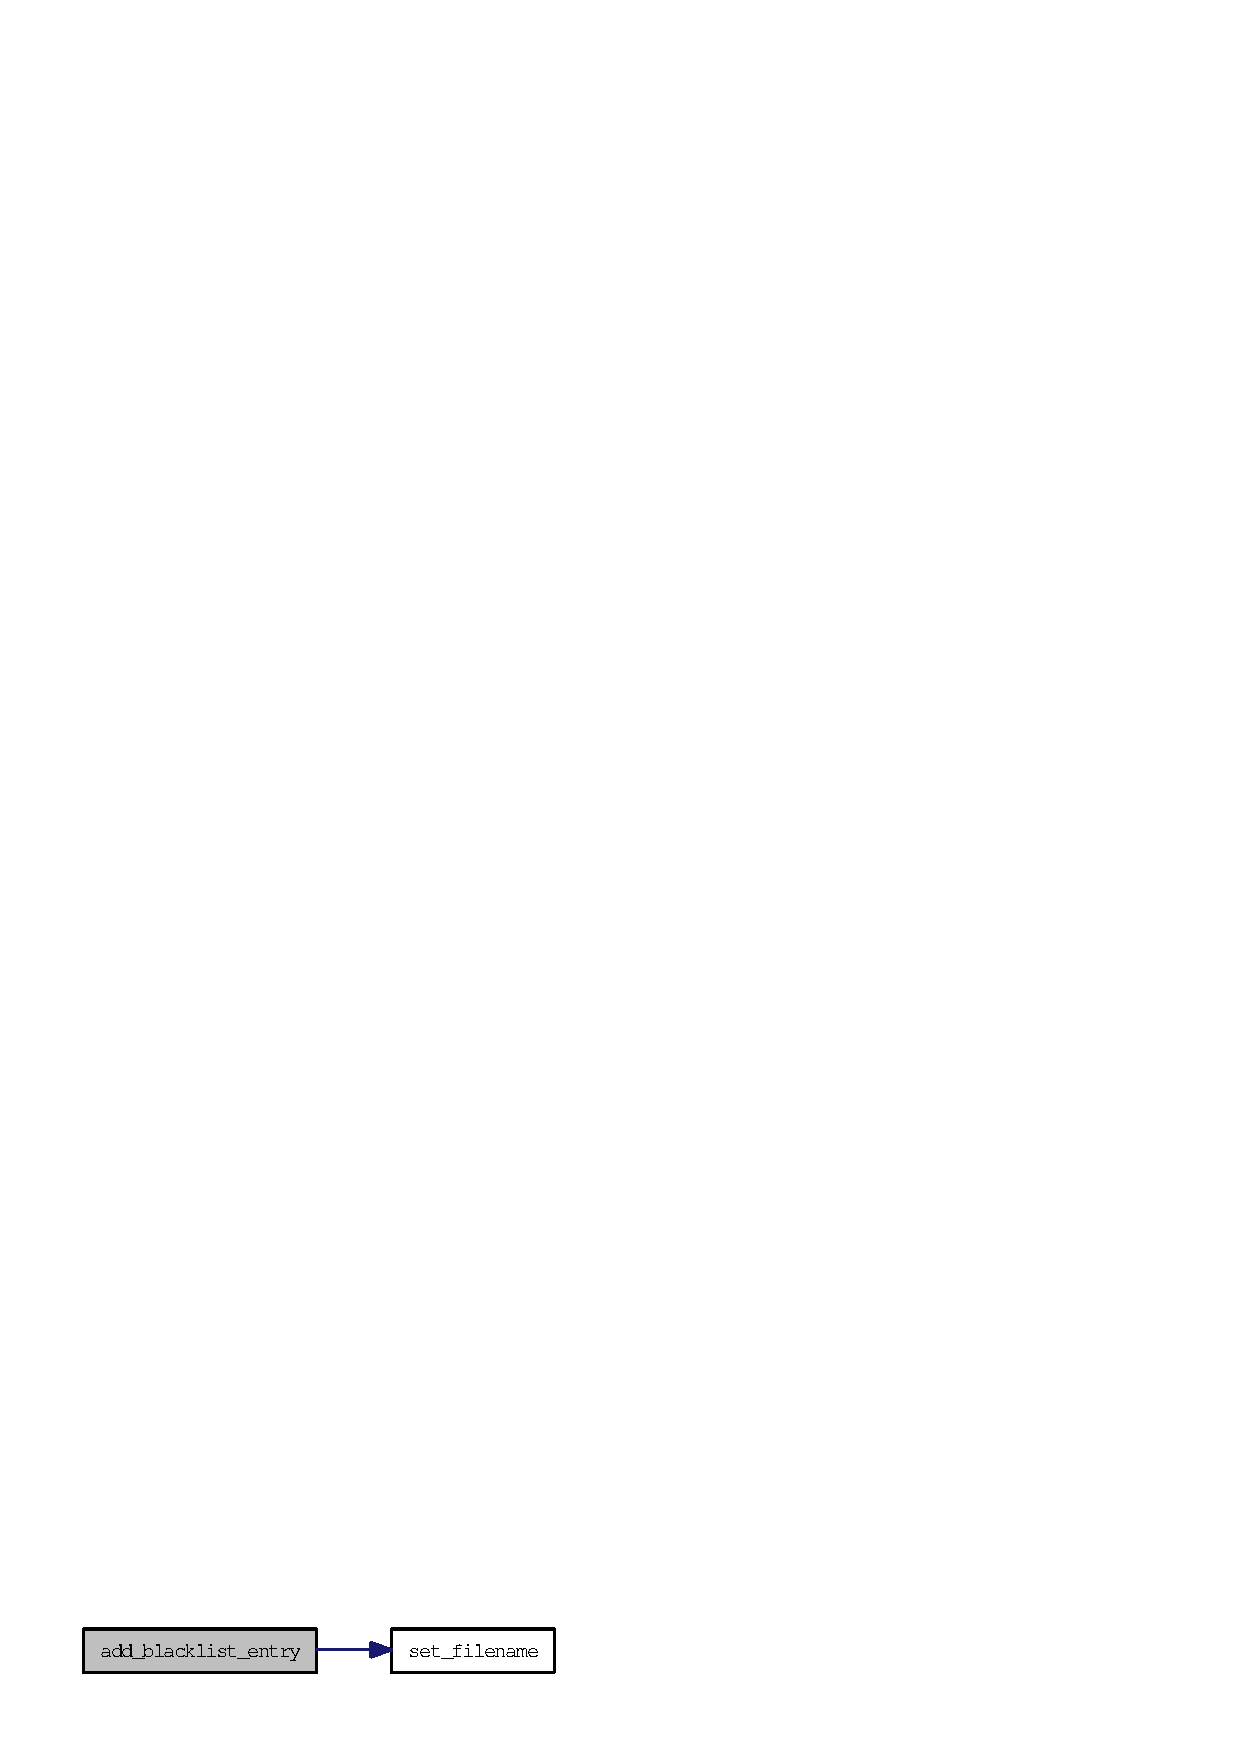
\includegraphics[width=135pt]{libphonefirewall_8h_36847ed3459e2a89038772ece42a017d_cgraph}
\end{center}
\end{figure}
\hypertarget{libphonefirewall_8h_eec16cb88eb546b1a2490e6716d75f8b}{
\index{libphonefirewall.h@{libphonefirewall.h}!add\_\-whitelist\_\-entry@{add\_\-whitelist\_\-entry}}
\index{add\_\-whitelist\_\-entry@{add\_\-whitelist\_\-entry}!libphonefirewall.h@{libphonefirewall.h}}
\subsubsection{\setlength{\rightskip}{0pt plus 5cm}int add\_\-whitelist\_\-entry (int {\em country\_\-code}, int {\em area\_\-code}, unsigned long long {\em number}, char $\ast$ {\em name}, char $\ast$ {\em reason}, int {\em priority})}}
\label{libphonefirewall_8h_eec16cb88eb546b1a2490e6716d75f8b}


Add a number to the whitelist. The number will be accepted after that.

\begin{Desc}
\item[Parameters:]
\begin{description}
\item[{\em country\_\-code}]The country code (for example 39 for Italy, 43 for Austria, and so one) \item[{\em area\_\-code}]The area code which indicates your mobile operator. \item[{\em number}]The telephone number of the person. \item[{\em name}]The name of the person. \item[{\em reason}]Why you have blocked this person. \item[{\em priority}]Gives the entry a priority. 0 is standard. If the priority is higher the value will be also blocked/accepted if a higher priority is choosen.\end{description}
\end{Desc}
\begin{Desc}
\item[Returns:]If all goes well 0 (zero) otherwise an errno code. \end{Desc}


Definition at line 53 of file phonefirewall\_\-administration.c.

References DELIM, filename, set\_\-filename(), and WHITELIST\_\-PREFIX.

Here is the call graph for this function:\nopagebreak
\begin{figure}[H]
\begin{center}
\leavevmode
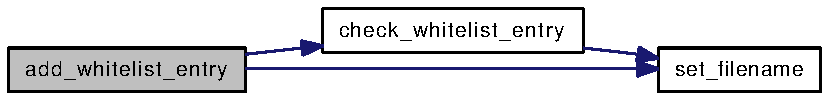
\includegraphics[width=136pt]{libphonefirewall_8h_eec16cb88eb546b1a2490e6716d75f8b_cgraph}
\end{center}
\end{figure}
\hypertarget{libphonefirewall_8h_651cdd0245f20256305b40f13bb9df2d}{
\index{libphonefirewall.h@{libphonefirewall.h}!check\_\-blacklist\_\-entry@{check\_\-blacklist\_\-entry}}
\index{check\_\-blacklist\_\-entry@{check\_\-blacklist\_\-entry}!libphonefirewall.h@{libphonefirewall.h}}
\subsubsection{\setlength{\rightskip}{0pt plus 5cm}char$\ast$ check\_\-blacklist\_\-entry (int {\em country\_\-code}, int {\em area\_\-code}, unsigned long long {\em number}, int {\em priority})}}
\label{libphonefirewall_8h_651cdd0245f20256305b40f13bb9df2d}


Checks if a number is on the blacklist.

\begin{Desc}
\item[Parameters:]
\begin{description}
\item[{\em country\_\-code}]The country code (for example 39 for Italy, 43 for Austria, and so one) \item[{\em area\_\-code}]The area code which indicates your mobile operator. \item[{\em number}]The telephone number of the person. \item[{\em priority}]Gives the entry a priority. 0 is standard. If the priority is higher the value will be also blocked/accepted if a higher priority is choosen.\end{description}
\end{Desc}
\begin{Desc}
\item[Returns:]If noting is found NULL, otherwise the number. \end{Desc}


Definition at line 74 of file phonefirewall\_\-administration.c.

References BLACKLIST\_\-PREFIX, DELIM, filename, MAX\_\-LINE\_\-LENGTH, and set\_\-filename().

Here is the call graph for this function:\nopagebreak
\begin{figure}[H]
\begin{center}
\leavevmode
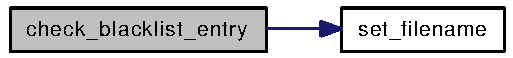
\includegraphics[width=141pt]{libphonefirewall_8h_651cdd0245f20256305b40f13bb9df2d_cgraph}
\end{center}
\end{figure}
\hypertarget{libphonefirewall_8h_032c45d6c7830492ddeaa8cabfc845c3}{
\index{libphonefirewall.h@{libphonefirewall.h}!check\_\-whitelist\_\-entry@{check\_\-whitelist\_\-entry}}
\index{check\_\-whitelist\_\-entry@{check\_\-whitelist\_\-entry}!libphonefirewall.h@{libphonefirewall.h}}
\subsubsection{\setlength{\rightskip}{0pt plus 5cm}char$\ast$ check\_\-whitelist\_\-entry (int {\em country\_\-code}, int {\em area\_\-code}, unsigned long long {\em number}, int {\em priority})}}
\label{libphonefirewall_8h_032c45d6c7830492ddeaa8cabfc845c3}


Checks if a number is on the whitelist.

\begin{Desc}
\item[Parameters:]
\begin{description}
\item[{\em country\_\-code}]The country code (for example 39 for Italy, 43 for Austria, and so one) \item[{\em area\_\-code}]The area code which indicates your mobile operator. \item[{\em number}]The telephone number of the person. \item[{\em priority}]Gives the entry a priority. 0 is standard. If the priority is higher the value will be also blocked/accepted if a higher priority is choosen.\end{description}
\end{Desc}
\begin{Desc}
\item[Returns:]If noting is found NULL, otherwise the number. \end{Desc}


Definition at line 105 of file phonefirewall\_\-administration.c.

References DELIM, filename, MAX\_\-LINE\_\-LENGTH, set\_\-filename(), and WHITELIST\_\-PREFIX.

Here is the call graph for this function:\nopagebreak
\begin{figure}[H]
\begin{center}
\leavevmode
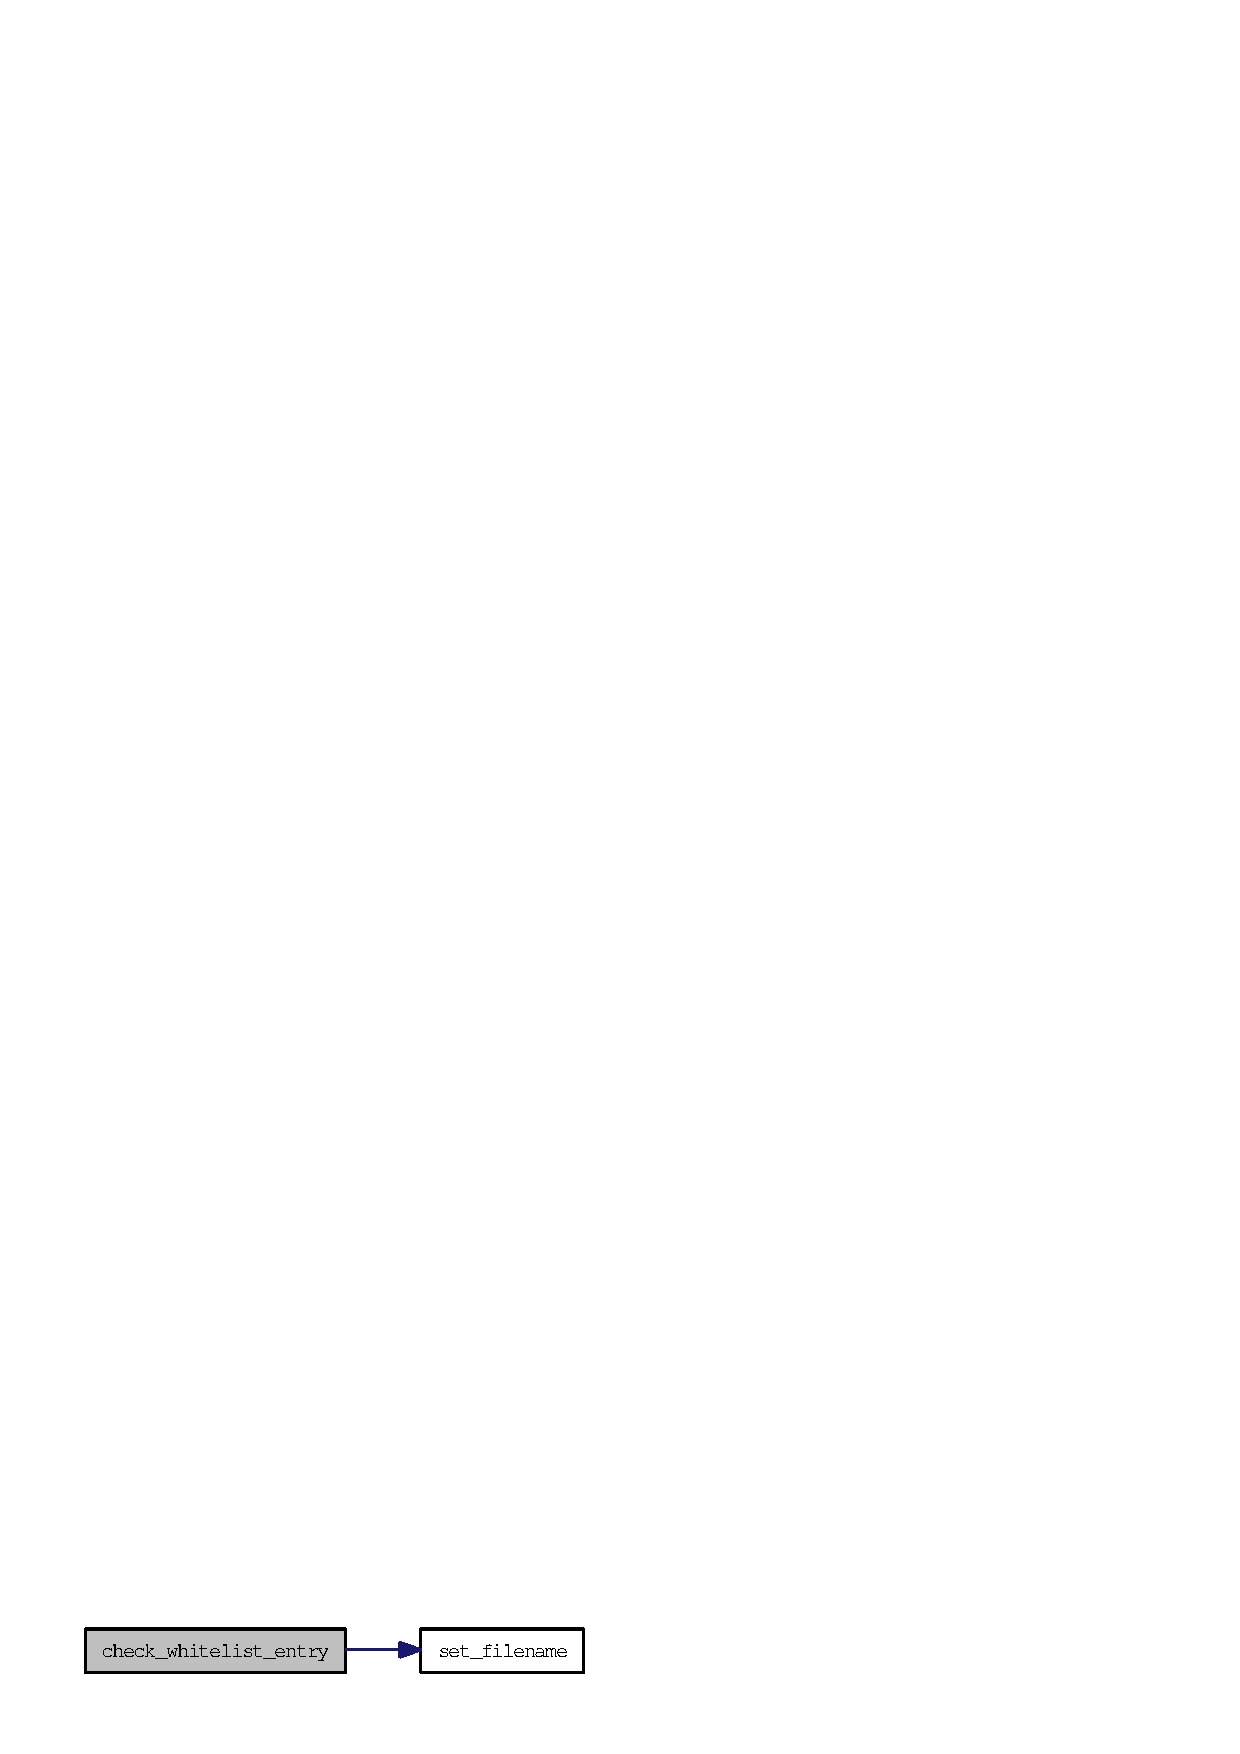
\includegraphics[width=142pt]{libphonefirewall_8h_032c45d6c7830492ddeaa8cabfc845c3_cgraph}
\end{center}
\end{figure}
\hypertarget{libphonefirewall_8h_e6c567f38aaa0eaa9db3eb13e32cdbbd}{
\index{libphonefirewall.h@{libphonefirewall.h}!rm\_\-blacklist\_\-entry@{rm\_\-blacklist\_\-entry}}
\index{rm\_\-blacklist\_\-entry@{rm\_\-blacklist\_\-entry}!libphonefirewall.h@{libphonefirewall.h}}
\subsubsection{\setlength{\rightskip}{0pt plus 5cm}int rm\_\-blacklist\_\-entry (unsigned long long {\em number})}}
\label{libphonefirewall_8h_e6c567f38aaa0eaa9db3eb13e32cdbbd}


Removes a blocked number from the blacklist.

\begin{Desc}
\item[Parameters:]
\begin{description}
\item[{\em number}]The number which will be deleted.\end{description}
\end{Desc}
\begin{Desc}
\item[Returns:]If all goes right 0, otherwise an error code. \end{Desc}


Definition at line 66 of file phonefirewall\_\-administration.c.\hypertarget{libphonefirewall_8h_e8a4ee30cf26b05a55680dc3a972f1a4}{
\index{libphonefirewall.h@{libphonefirewall.h}!rm\_\-whitelist\_\-entry@{rm\_\-whitelist\_\-entry}}
\index{rm\_\-whitelist\_\-entry@{rm\_\-whitelist\_\-entry}!libphonefirewall.h@{libphonefirewall.h}}
\subsubsection{\setlength{\rightskip}{0pt plus 5cm}int rm\_\-whitelist\_\-entry (unsigned long long {\em number})}}
\label{libphonefirewall_8h_e8a4ee30cf26b05a55680dc3a972f1a4}


Removes a accepted number from the whitelist.

\begin{Desc}
\item[Parameters:]
\begin{description}
\item[{\em number}]The number which will be deleted.\end{description}
\end{Desc}
\begin{Desc}
\item[Returns:]If all goes right 0, otherwise an error code. \end{Desc}


Definition at line 70 of file phonefirewall\_\-administration.c.
\hypertarget{phonefirewall__administration_8c}{
\section{phonefirewall\_\-administration.c File Reference}
\label{phonefirewall__administration_8c}\index{phonefirewall\_\-administration.c@{phonefirewall\_\-administration.c}}
}
{\tt \#include $<$stdio.h$>$}\par
{\tt \#include $<$stdlib.h$>$}\par
{\tt \#include $<$errno.h$>$}\par
{\tt \#include $<$string.h$>$}\par
{\tt \#include \char`\"{}libphonefirewall.h\char`\"{}}\par


Include dependency graph for phonefirewall\_\-administration.c:\nopagebreak
\begin{figure}[H]
\begin{center}
\leavevmode
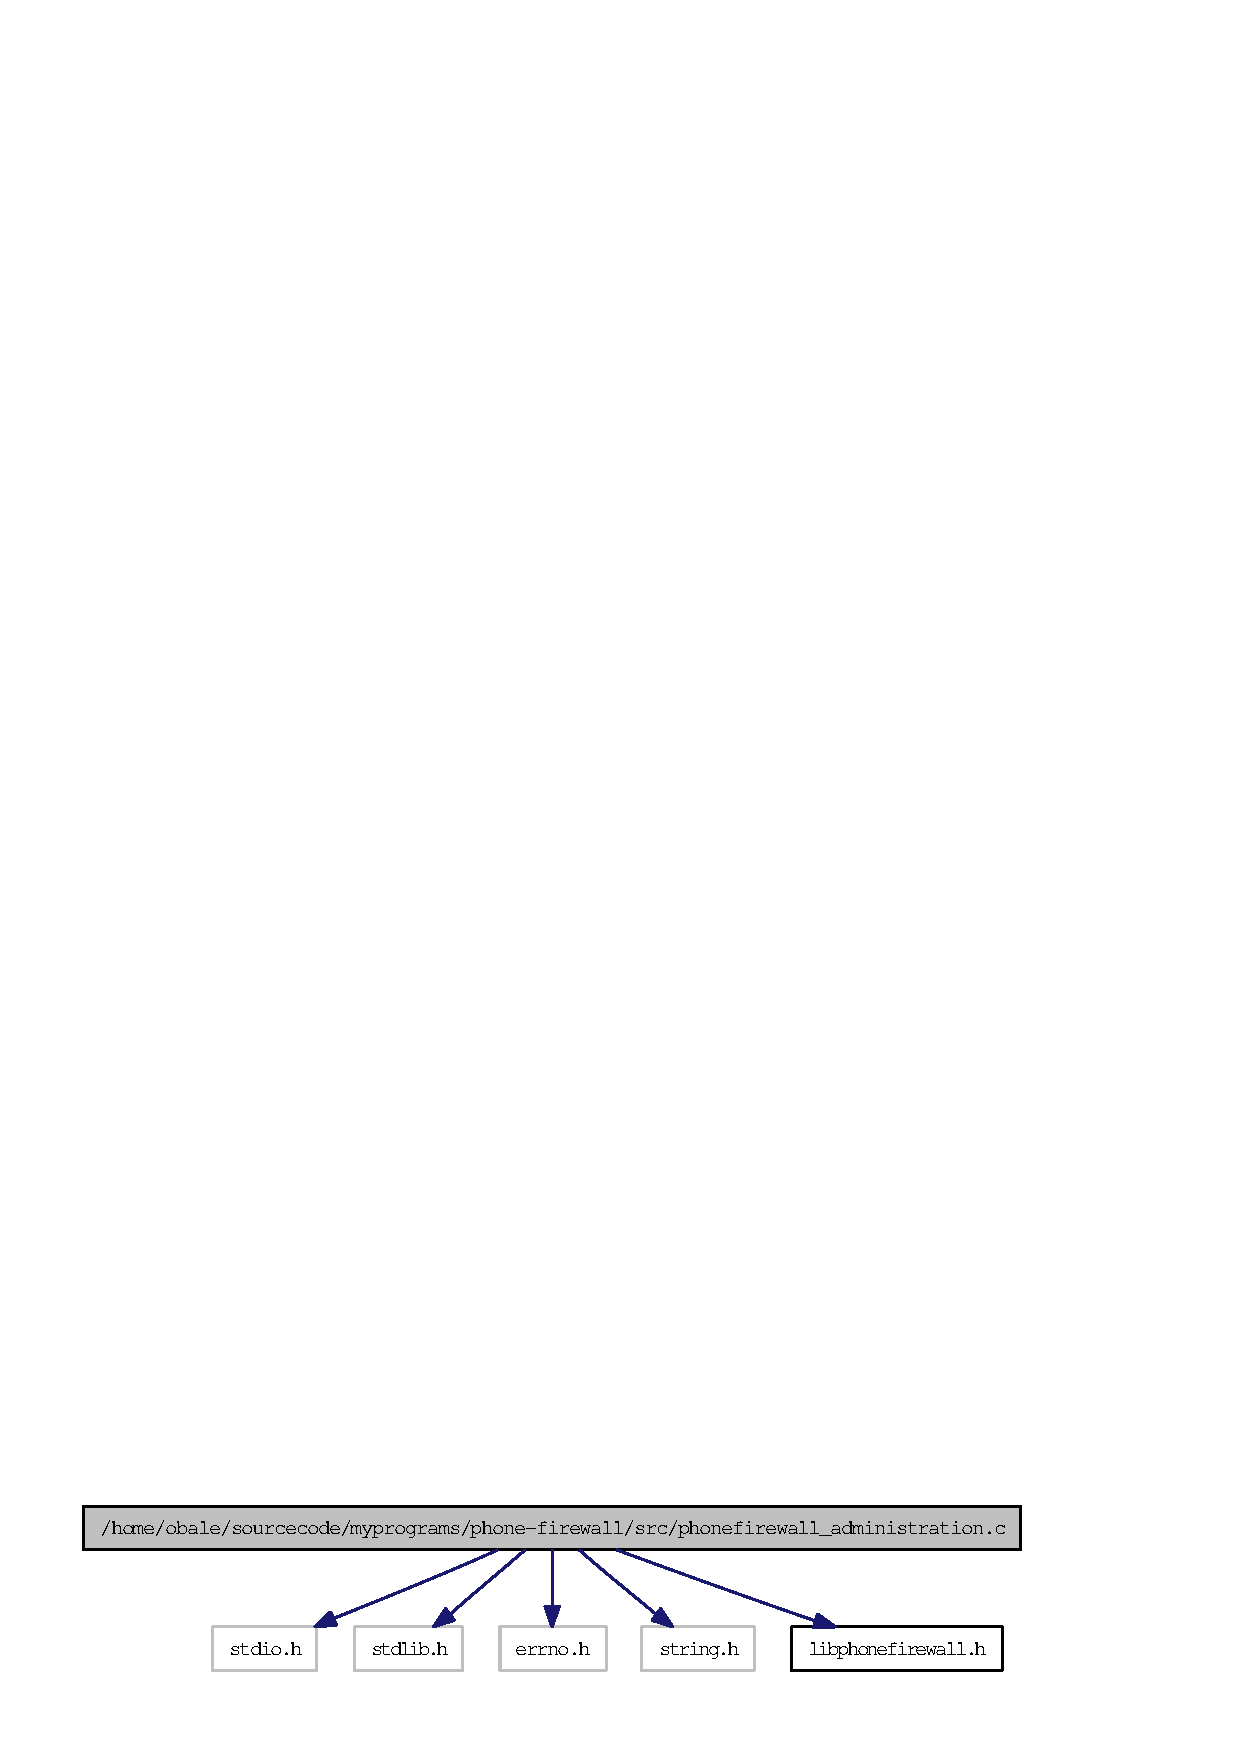
\includegraphics[width=211pt]{phonefirewall__administration_8c__incl}
\end{center}
\end{figure}
\subsection*{Defines}
\begin{CompactItemize}
\item 
\#define \hyperlink{phonefirewall__administration_8c_c0120f27d973f4ea90962305431fedce}{BLACKLIST\_\-PREFIX}~\char`\"{}db/blacklist\_\-\char`\"{}
\item 
\#define \hyperlink{phonefirewall__administration_8c_b5b8614b1e4d5e316cc4a8102ce9636c}{WHITELIST\_\-PREFIX}~\char`\"{}db/whitelist\_\-\char`\"{}
\item 
\#define \hyperlink{phonefirewall__administration_8c_03bc2a42c1399400ae0d103f5ada724c}{FILENAME\_\-SIZE}~256
\end{CompactItemize}
\subsection*{Functions}
\begin{CompactItemize}
\item 
int \hyperlink{phonefirewall__administration_8c_d42187af304bf25d98f7f7f76853c6f7}{set\_\-filename} (char $\ast$prefix, int country\_\-code, int area\_\-code)
\item 
int \hyperlink{phonefirewall__administration_8c_36847ed3459e2a89038772ece42a017d}{add\_\-blacklist\_\-entry} (int country\_\-code, int area\_\-code, unsigned long long number, char $\ast$name, char $\ast$reason, int priority)
\item 
int \hyperlink{phonefirewall__administration_8c_eec16cb88eb546b1a2490e6716d75f8b}{add\_\-whitelist\_\-entry} (int country\_\-code, int area\_\-code, unsigned long long number, char $\ast$name, char $\ast$reason, int priority)
\item 
int \hyperlink{phonefirewall__administration_8c_e6c567f38aaa0eaa9db3eb13e32cdbbd}{rm\_\-blacklist\_\-entry} (unsigned long long number)
\item 
int \hyperlink{phonefirewall__administration_8c_e8a4ee30cf26b05a55680dc3a972f1a4}{rm\_\-whitelist\_\-entry} (unsigned long long number)
\item 
char $\ast$ \hyperlink{phonefirewall__administration_8c_651cdd0245f20256305b40f13bb9df2d}{check\_\-blacklist\_\-entry} (int country\_\-code, int area\_\-code, unsigned long long number, int priority)
\item 
char $\ast$ \hyperlink{phonefirewall__administration_8c_032c45d6c7830492ddeaa8cabfc845c3}{check\_\-whitelist\_\-entry} (int country\_\-code, int area\_\-code, unsigned long long number, int priority)
\end{CompactItemize}
\subsection*{Variables}
\begin{CompactItemize}
\item 
static char $\ast$ \hyperlink{phonefirewall__administration_8c_6c7d3710dd8e86998206dad075d6fc27}{DELIM} = \char`\"{}::\char`\"{}
\item 
char \hyperlink{phonefirewall__administration_8c_89707f7a91e271cac7f8e4e2a0be0006}{filename} \mbox{[}FILENAME\_\-SIZE\mbox{]}
\end{CompactItemize}


\subsection{Define Documentation}
\hypertarget{phonefirewall__administration_8c_c0120f27d973f4ea90962305431fedce}{
\index{phonefirewall\_\-administration.c@{phonefirewall\_\-administration.c}!BLACKLIST\_\-PREFIX@{BLACKLIST\_\-PREFIX}}
\index{BLACKLIST\_\-PREFIX@{BLACKLIST\_\-PREFIX}!phonefirewall_administration.c@{phonefirewall\_\-administration.c}}
\subsubsection{\setlength{\rightskip}{0pt plus 5cm}\#define BLACKLIST\_\-PREFIX~\char`\"{}db/blacklist\_\-\char`\"{}}}
\label{phonefirewall__administration_8c_c0120f27d973f4ea90962305431fedce}




Definition at line 26 of file phonefirewall\_\-administration.c.

Referenced by add\_\-blacklist\_\-entry(), and check\_\-blacklist\_\-entry().\hypertarget{phonefirewall__administration_8c_03bc2a42c1399400ae0d103f5ada724c}{
\index{phonefirewall\_\-administration.c@{phonefirewall\_\-administration.c}!FILENAME\_\-SIZE@{FILENAME\_\-SIZE}}
\index{FILENAME\_\-SIZE@{FILENAME\_\-SIZE}!phonefirewall_administration.c@{phonefirewall\_\-administration.c}}
\subsubsection{\setlength{\rightskip}{0pt plus 5cm}\#define FILENAME\_\-SIZE~256}}
\label{phonefirewall__administration_8c_03bc2a42c1399400ae0d103f5ada724c}




Definition at line 28 of file phonefirewall\_\-administration.c.\hypertarget{phonefirewall__administration_8c_b5b8614b1e4d5e316cc4a8102ce9636c}{
\index{phonefirewall\_\-administration.c@{phonefirewall\_\-administration.c}!WHITELIST\_\-PREFIX@{WHITELIST\_\-PREFIX}}
\index{WHITELIST\_\-PREFIX@{WHITELIST\_\-PREFIX}!phonefirewall_administration.c@{phonefirewall\_\-administration.c}}
\subsubsection{\setlength{\rightskip}{0pt plus 5cm}\#define WHITELIST\_\-PREFIX~\char`\"{}db/whitelist\_\-\char`\"{}}}
\label{phonefirewall__administration_8c_b5b8614b1e4d5e316cc4a8102ce9636c}




Definition at line 27 of file phonefirewall\_\-administration.c.

Referenced by add\_\-whitelist\_\-entry(), and check\_\-whitelist\_\-entry().

\subsection{Function Documentation}
\hypertarget{phonefirewall__administration_8c_36847ed3459e2a89038772ece42a017d}{
\index{phonefirewall\_\-administration.c@{phonefirewall\_\-administration.c}!add\_\-blacklist\_\-entry@{add\_\-blacklist\_\-entry}}
\index{add\_\-blacklist\_\-entry@{add\_\-blacklist\_\-entry}!phonefirewall_administration.c@{phonefirewall\_\-administration.c}}
\subsubsection{\setlength{\rightskip}{0pt plus 5cm}int add\_\-blacklist\_\-entry (int {\em country\_\-code}, int {\em area\_\-code}, unsigned long long {\em number}, char $\ast$ {\em name}, char $\ast$ {\em reason}, int {\em priority})}}
\label{phonefirewall__administration_8c_36847ed3459e2a89038772ece42a017d}


Add a number to the blacklist. The number will be blocked after that.

\begin{Desc}
\item[Parameters:]
\begin{description}
\item[{\em country\_\-code}]The country code (for example 39 for Italy, 43 for Austria, and so one) \item[{\em area\_\-code}]The area code which indicates your mobile operator. \item[{\em number}]The telephone number of the person (without country and area code. \item[{\em name}]The name of the person. \item[{\em reason}]Why you have blocked this person. \item[{\em priority}]Gives the \hyperlink{structentry}{entry} a priority. 0 is standard. If the priority is higher the value will be also blocked/accepted if a higher priority is choosen.\end{description}
\end{Desc}
\begin{Desc}
\item[Returns:]If all goes well 0 (zero) otherwise an errno code. \end{Desc}


Definition at line 40 of file phonefirewall\_\-administration.c.

References BLACKLIST\_\-PREFIX, DELIM, filename, and set\_\-filename().

Here is the call graph for this function:\nopagebreak
\begin{figure}[H]
\begin{center}
\leavevmode
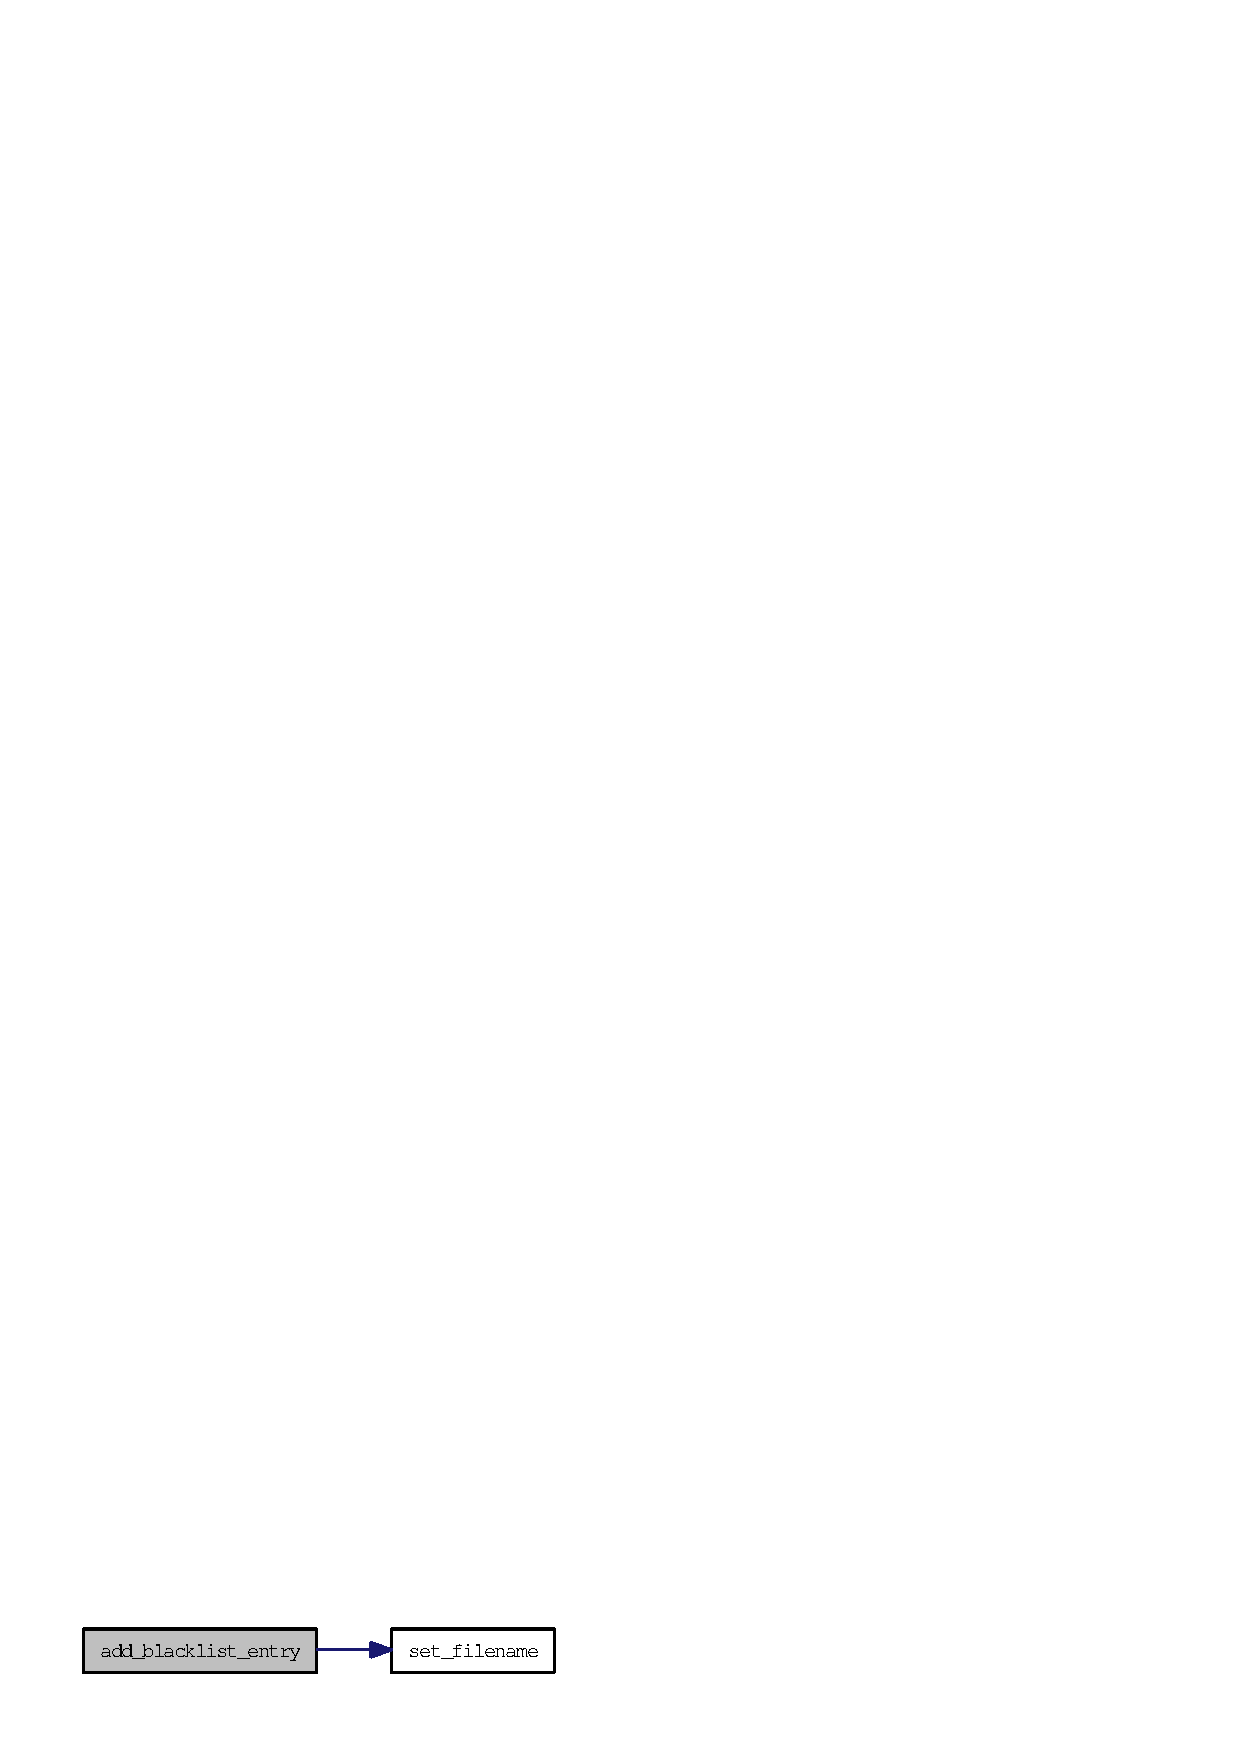
\includegraphics[width=135pt]{phonefirewall__administration_8c_36847ed3459e2a89038772ece42a017d_cgraph}
\end{center}
\end{figure}
\hypertarget{phonefirewall__administration_8c_eec16cb88eb546b1a2490e6716d75f8b}{
\index{phonefirewall\_\-administration.c@{phonefirewall\_\-administration.c}!add\_\-whitelist\_\-entry@{add\_\-whitelist\_\-entry}}
\index{add\_\-whitelist\_\-entry@{add\_\-whitelist\_\-entry}!phonefirewall_administration.c@{phonefirewall\_\-administration.c}}
\subsubsection{\setlength{\rightskip}{0pt plus 5cm}int add\_\-whitelist\_\-entry (int {\em country\_\-code}, int {\em area\_\-code}, unsigned long long {\em number}, char $\ast$ {\em name}, char $\ast$ {\em reason}, int {\em priority})}}
\label{phonefirewall__administration_8c_eec16cb88eb546b1a2490e6716d75f8b}


Add a number to the whitelist. The number will be accepted after that.

\begin{Desc}
\item[Parameters:]
\begin{description}
\item[{\em country\_\-code}]The country code (for example 39 for Italy, 43 for Austria, and so one) \item[{\em area\_\-code}]The area code which indicates your mobile operator. \item[{\em number}]The telephone number of the person (without country and area code. \item[{\em name}]The name of the person. \item[{\em reason}]Why you have blocked this person. \item[{\em priority}]Gives the \hyperlink{structentry}{entry} a priority. 0 is standard. If the priority is higher the value will be also blocked/accepted if a higher priority is choosen.\end{description}
\end{Desc}
\begin{Desc}
\item[Returns:]If all goes well 0 (zero) otherwise an errno code. \end{Desc}


Definition at line 54 of file phonefirewall\_\-administration.c.

References DELIM, filename, set\_\-filename(), and WHITELIST\_\-PREFIX.

Here is the call graph for this function:\nopagebreak
\begin{figure}[H]
\begin{center}
\leavevmode
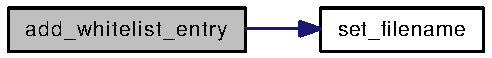
\includegraphics[width=136pt]{phonefirewall__administration_8c_eec16cb88eb546b1a2490e6716d75f8b_cgraph}
\end{center}
\end{figure}
\hypertarget{phonefirewall__administration_8c_651cdd0245f20256305b40f13bb9df2d}{
\index{phonefirewall\_\-administration.c@{phonefirewall\_\-administration.c}!check\_\-blacklist\_\-entry@{check\_\-blacklist\_\-entry}}
\index{check\_\-blacklist\_\-entry@{check\_\-blacklist\_\-entry}!phonefirewall_administration.c@{phonefirewall\_\-administration.c}}
\subsubsection{\setlength{\rightskip}{0pt plus 5cm}char$\ast$ check\_\-blacklist\_\-entry (int {\em country\_\-code}, int {\em area\_\-code}, unsigned long long {\em number}, int {\em priority})}}
\label{phonefirewall__administration_8c_651cdd0245f20256305b40f13bb9df2d}


Checks if a number is on the blacklist.

\begin{Desc}
\item[Parameters:]
\begin{description}
\item[{\em country\_\-code}]The country code (for example 39 for Italy, 43 for Austria, and so one) \item[{\em area\_\-code}]The area code which indicates your mobile operator. \item[{\em number}]The telephone number of the person (without country and area code. \item[{\em priority}]Gives the \hyperlink{structentry}{entry} a priority. 0 is standard. If the priority is higher the value will be also blocked/accepted if a higher priority is choosen.\end{description}
\end{Desc}
\begin{Desc}
\item[Returns:]If noting is found NULL, otherwise the number. \end{Desc}


Definition at line 76 of file phonefirewall\_\-administration.c.

References BLACKLIST\_\-PREFIX, DELIM, filename, MAX\_\-LINE\_\-LENGTH, and set\_\-filename().

Here is the call graph for this function:\nopagebreak
\begin{figure}[H]
\begin{center}
\leavevmode
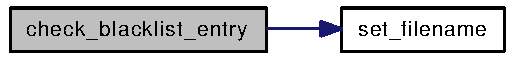
\includegraphics[width=141pt]{phonefirewall__administration_8c_651cdd0245f20256305b40f13bb9df2d_cgraph}
\end{center}
\end{figure}
\hypertarget{phonefirewall__administration_8c_032c45d6c7830492ddeaa8cabfc845c3}{
\index{phonefirewall\_\-administration.c@{phonefirewall\_\-administration.c}!check\_\-whitelist\_\-entry@{check\_\-whitelist\_\-entry}}
\index{check\_\-whitelist\_\-entry@{check\_\-whitelist\_\-entry}!phonefirewall_administration.c@{phonefirewall\_\-administration.c}}
\subsubsection{\setlength{\rightskip}{0pt plus 5cm}char$\ast$ check\_\-whitelist\_\-entry (int {\em country\_\-code}, int {\em area\_\-code}, unsigned long long {\em number}, int {\em priority})}}
\label{phonefirewall__administration_8c_032c45d6c7830492ddeaa8cabfc845c3}


Checks if a number is on the whitelist.

\begin{Desc}
\item[Parameters:]
\begin{description}
\item[{\em country\_\-code}]The country code (for example 39 for Italy, 43 for Austria, and so one) \item[{\em area\_\-code}]The area code which indicates your mobile operator. \item[{\em number}]The telephone number of the person (without country and area code. \item[{\em priority}]Gives the \hyperlink{structentry}{entry} a priority. 0 is standard. If the priority is higher the value will be also blocked/accepted if a higher priority is choosen.\end{description}
\end{Desc}
\begin{Desc}
\item[Returns:]If noting is found NULL, otherwise the number. \end{Desc}


Definition at line 110 of file phonefirewall\_\-administration.c.

References DELIM, filename, MAX\_\-LINE\_\-LENGTH, set\_\-filename(), and WHITELIST\_\-PREFIX.

Here is the call graph for this function:\nopagebreak
\begin{figure}[H]
\begin{center}
\leavevmode
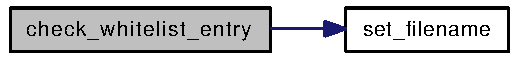
\includegraphics[width=142pt]{phonefirewall__administration_8c_032c45d6c7830492ddeaa8cabfc845c3_cgraph}
\end{center}
\end{figure}
\hypertarget{phonefirewall__administration_8c_e6c567f38aaa0eaa9db3eb13e32cdbbd}{
\index{phonefirewall\_\-administration.c@{phonefirewall\_\-administration.c}!rm\_\-blacklist\_\-entry@{rm\_\-blacklist\_\-entry}}
\index{rm\_\-blacklist\_\-entry@{rm\_\-blacklist\_\-entry}!phonefirewall_administration.c@{phonefirewall\_\-administration.c}}
\subsubsection{\setlength{\rightskip}{0pt plus 5cm}int rm\_\-blacklist\_\-entry (unsigned long long {\em number})}}
\label{phonefirewall__administration_8c_e6c567f38aaa0eaa9db3eb13e32cdbbd}


Removes a blocked number from the blacklist.

\begin{Desc}
\item[Parameters:]
\begin{description}
\item[{\em number}]The number which will be deleted.\end{description}
\end{Desc}
\begin{Desc}
\item[Returns:]If all goes right 0, otherwise an error code. \end{Desc}


Definition at line 68 of file phonefirewall\_\-administration.c.\hypertarget{phonefirewall__administration_8c_e8a4ee30cf26b05a55680dc3a972f1a4}{
\index{phonefirewall\_\-administration.c@{phonefirewall\_\-administration.c}!rm\_\-whitelist\_\-entry@{rm\_\-whitelist\_\-entry}}
\index{rm\_\-whitelist\_\-entry@{rm\_\-whitelist\_\-entry}!phonefirewall_administration.c@{phonefirewall\_\-administration.c}}
\subsubsection{\setlength{\rightskip}{0pt plus 5cm}int rm\_\-whitelist\_\-entry (unsigned long long {\em number})}}
\label{phonefirewall__administration_8c_e8a4ee30cf26b05a55680dc3a972f1a4}


Removes a accepted number from the whitelist.

\begin{Desc}
\item[Parameters:]
\begin{description}
\item[{\em number}]The number which will be deleted.\end{description}
\end{Desc}
\begin{Desc}
\item[Returns:]If all goes right 0, otherwise an error code. \end{Desc}


Definition at line 72 of file phonefirewall\_\-administration.c.\hypertarget{phonefirewall__administration_8c_d42187af304bf25d98f7f7f76853c6f7}{
\index{phonefirewall\_\-administration.c@{phonefirewall\_\-administration.c}!set\_\-filename@{set\_\-filename}}
\index{set\_\-filename@{set\_\-filename}!phonefirewall_administration.c@{phonefirewall\_\-administration.c}}
\subsubsection{\setlength{\rightskip}{0pt plus 5cm}int set\_\-filename (char $\ast$ {\em prefix}, int {\em country\_\-code}, int {\em area\_\-code})}}
\label{phonefirewall__administration_8c_d42187af304bf25d98f7f7f76853c6f7}




Definition at line 34 of file phonefirewall\_\-administration.c.

References filename.

Referenced by add\_\-blacklist\_\-entry(), add\_\-whitelist\_\-entry(), check\_\-blacklist\_\-entry(), and check\_\-whitelist\_\-entry().

Here is the caller graph for this function:\nopagebreak
\begin{figure}[H]
\begin{center}
\leavevmode
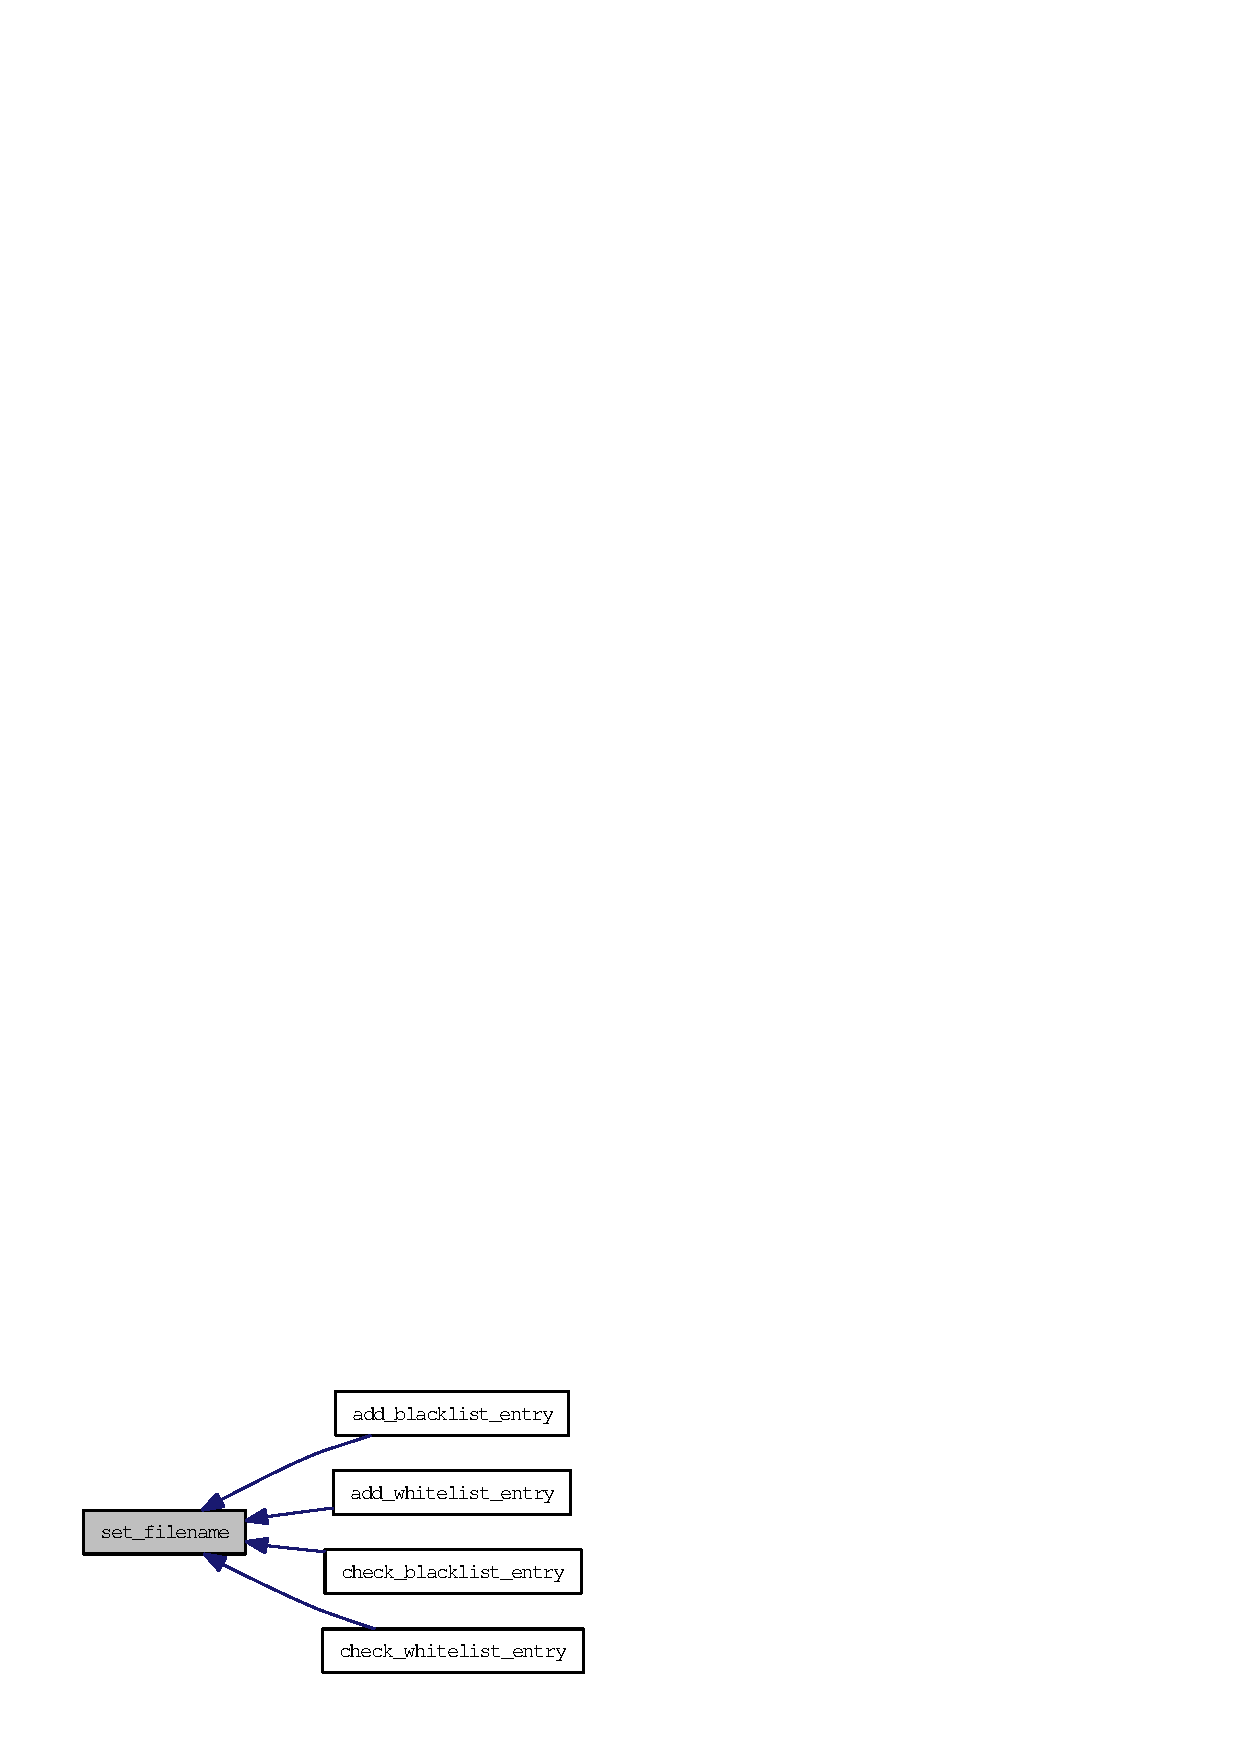
\includegraphics[width=142pt]{phonefirewall__administration_8c_d42187af304bf25d98f7f7f76853c6f7_icgraph}
\end{center}
\end{figure}


\subsection{Variable Documentation}
\hypertarget{phonefirewall__administration_8c_6c7d3710dd8e86998206dad075d6fc27}{
\index{phonefirewall\_\-administration.c@{phonefirewall\_\-administration.c}!DELIM@{DELIM}}
\index{DELIM@{DELIM}!phonefirewall_administration.c@{phonefirewall\_\-administration.c}}
\subsubsection{\setlength{\rightskip}{0pt plus 5cm}char$\ast$ {\bf DELIM} = \char`\"{}::\char`\"{}\hspace{0.3cm}{\tt  \mbox{[}static\mbox{]}}}}
\label{phonefirewall__administration_8c_6c7d3710dd8e86998206dad075d6fc27}




Definition at line 30 of file phonefirewall\_\-administration.c.

Referenced by add\_\-blacklist\_\-entry(), add\_\-whitelist\_\-entry(), check\_\-blacklist\_\-entry(), and check\_\-whitelist\_\-entry().\hypertarget{phonefirewall__administration_8c_89707f7a91e271cac7f8e4e2a0be0006}{
\index{phonefirewall\_\-administration.c@{phonefirewall\_\-administration.c}!filename@{filename}}
\index{filename@{filename}!phonefirewall_administration.c@{phonefirewall\_\-administration.c}}
\subsubsection{\setlength{\rightskip}{0pt plus 5cm}char {\bf filename}\mbox{[}FILENAME\_\-SIZE\mbox{]}}}
\label{phonefirewall__administration_8c_89707f7a91e271cac7f8e4e2a0be0006}




Definition at line 32 of file phonefirewall\_\-administration.c.

Referenced by add\_\-blacklist\_\-entry(), add\_\-whitelist\_\-entry(), check\_\-blacklist\_\-entry(), check\_\-whitelist\_\-entry(), and set\_\-filename().
\printindex
\end{document}
